\documentclass{article}

\usepackage{graphicx}

\voffset = -50pt
\textheight = 650pt

\begin{document}

\thispagestyle{empty}

\section*{Design of a Very Simple Game on Paper}

The goal in this game is to go from START to END using the following rules:

\begin{enumerate}

  \item The player begins at ``START'' with five hit points (HP) strength set to
    zero;

  \item The player can move and direction and any number of steps, however doors
    and enemies block her/his way;

  \item A door can be opened with the key of door's colour;

  \item In order to pass an enemy the player should defeat it using two dices.
    If the player rolls less than the enemy's strength (shown in the cell where
    the enemy resides) then the players loses 1 HP, otherwise the enemy dies
    and the player's strenght increases by one;

  \item Picking up the flask grants the player 2 HP, the axe gives 1 strenght
    and sword 2 strength points;

  \item The game ends if player's HP goes to zero (losing) or the player
    reaches ``END'' (winning).

\end{enumerate}

A degree of difficulty by chance is not very high in the beginning. The chance
involves either to defeat the enemy or lose 1 HP. The enemies become stronger
faster than the player.

Skill is to figure out the order of picking up the keys and defeating enemies,
as well as deciding whether to for the axe.

\begin{figure}[ht]
  \centering
  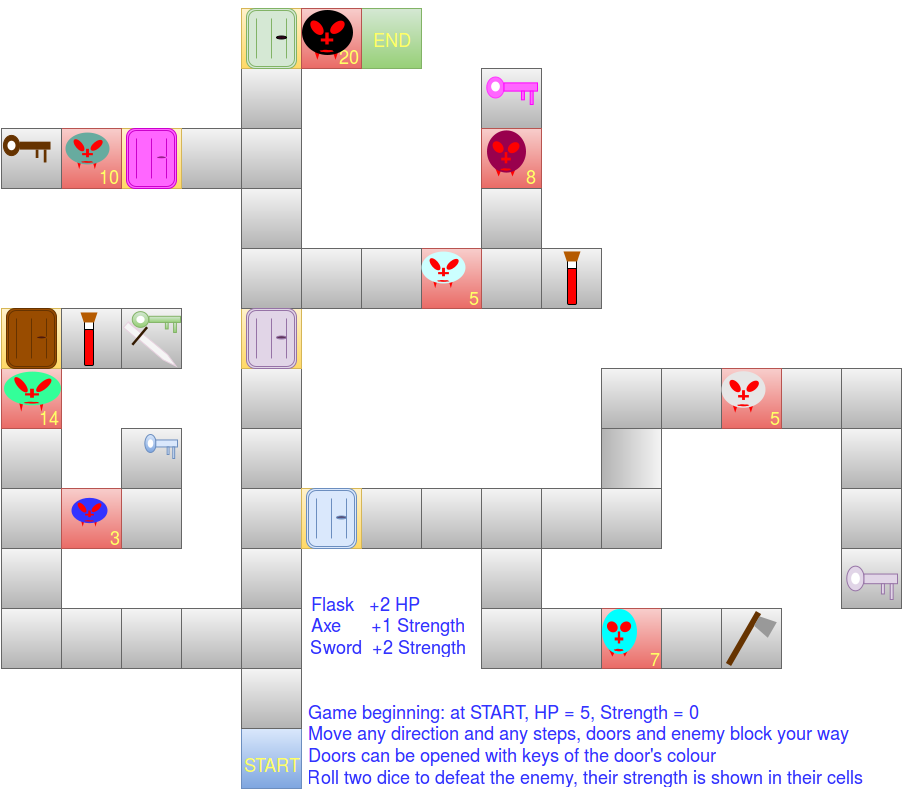
\includegraphics[width=\textwidth]{simpleGameDesign.png}
\end{figure}

\end{document}
